%% chapter15_slides.tex
%% Beamer slides for Chapter 15: Improved e-value thresholds under additional conditions
%% "Hypothesis Testing with E-Values" by Aaditya Ramdas and Ruodu Wang (arXiv:2410.23614)
%% Reader-friendly style: intuition first, step-by-step derivations, worked numeric example
%% Compiled with: pdflatex -interaction=nonstopmode chapter15_slides.tex  (twice)
\documentclass[aspectratio=169,10pt]{beamer}

\usetheme{Madrid}
\usecolortheme{seahorse}
\usefonttheme{professionalfonts}

%% ── Packages ──────────────────────────────────────────────────────────────
\usepackage{amsmath,amssymb,amsfonts}
\usepackage{mathtools}
\usepackage{graphicx}
\usepackage{booktabs}
\usepackage{xcolor}
\usepackage{listings}

\graphicspath{{figures/}}

%% ── Python listing style ─────────────────────────────────────────────────
\lstdefinestyle{pycode}{
  language=Python,
  basicstyle=\ttfamily\scriptsize,
  numbers=left,
  numberstyle=\tiny\color{gray},
  frame=single,
  backgroundcolor=\color{gray!7},
  keywordstyle=\color{blue!70!black}\bfseries,
  commentstyle=\color{green!50!black}\itshape,
  stringstyle=\color{orange!80!black},
  showstringspaces=false,
  breaklines=true,
  tabsize=2,
  xleftmargin=1.5em,
  framexleftmargin=1.5em,
  aboveskip=4pt,
  belowskip=4pt,
}
\lstset{style=pycode}

%% ── Metadata ─────────────────────────────────────────────────────────────
\title[E-Values -- Ch.15]{Hypothesis Testing with E-Values}
\subtitle{Chapter 15: Improved E-Value Thresholds under Additional Conditions}
\author{Based on Ramdas \& Wang}
\date{}

\setbeamertemplate{footline}[frame number]
\setbeamertemplate{navigation symbols}{}

%% ── Macros ────────────────────────────────────────────────────────────────
\newcommand{\PP}{\mathbb{P}}
\newcommand{\EE}{\mathbb{E}}
\newcommand{\RR}{\mathbb{R}}
\newcommand{\calE}{\mathcal{E}}
\newcommand{\calX}{\mathcal{X}}
\newcommand{\frakE}{\mathfrak{E}}
\newcommand{\ED}{\mathcal{E}_{\mathrm{D}}}
\newcommand{\EDone}{\mathcal{E}_{\mathrm{D}>1}}
\newcommand{\EU}{\mathcal{E}_{\mathrm{U}}}
\newcommand{\ELS}{\mathcal{E}_{\mathrm{LS}}}
\newcommand{\ELU}{\mathcal{E}_{\mathrm{LU}}}
\newcommand{\ELDzero}{\mathcal{E}_{\mathrm{LD}>0}}
\newcommand{\ELD}{\mathcal{E}_{\mathrm{LD}}}
\newcommand{\ELUS}{\mathcal{E}_{\mathrm{LUS}}}
\newcommand{\ELN}{\mathcal{E}_{\mathrm{LN}}}

\begin{document}

%% =========================================================================
\begin{frame}
  \titlepage
\end{frame}

%% =========================================================================
\begin{frame}{Where we are}
  \begin{itemize}
    \item \textbf{Chapters 2, 8, 11} gave us the universal safety net: for \emph{any} e-variable $E$ (valid under a null $\PP$), Markov's inequality gives $\PP(E\ge 1/\alpha)\le\alpha$. Rejecting when $E\ge 1/\alpha$ is always a valid level-$\alpha$ test, no matter how weird $E$'s distribution is.
    \item That worst-case guarantee is bought at a price: if we \emph{happen to know something extra} about the shape of $E$'s distribution, the threshold $1/\alpha$ is needlessly conservative.
    \item \textbf{Chapter 15} asks: what extra, checkable, distribution-shape assumptions let us reject at a \emph{smaller} threshold than $1/\alpha$ -- giving a strictly more powerful test while remaining exactly as valid?
    \item Roadmap:
    \begin{itemize}
      \item 15.1: the general machinery -- the quantity $R_\gamma(\calE)$ and the resulting threshold $T_\alpha(\calE)$, for any restricted class $\calE$ of e-variables;
      \item 15.2: \textbf{comonotonic} e-variables -- families that all move together;
      \item 15.3: \textbf{density conditions} -- decreasing or unimodal densities;
      \item 15.4: conditions on the \textbf{log} of the e-variable, motivated by products of e-values (e-processes) and the CLT.
    \end{itemize}
    \item Throughout, we fix a single (atomless) null $\PP$; composite nulls just require the shape assumption to hold under every null distribution.
  \end{itemize}
\end{frame}

%% =========================================================================
\begin{frame}[allowframebreaks]{Notation you'll need}
  \begin{block}{Recap: the Markov/Ville threshold (Chapter 2, Proposition 2.1)}
    For \emph{any} e-variable $E$ (i.e.\ $E\ge0$, $\EE^\PP[E]\le1$) and any $\alpha\in(0,1)$,
    \[
      \PP(E\ge 1/\alpha)\;\le\;\alpha.
    \]
    So ``reject $H_0$ iff $E\ge 1/\alpha$'' is always a valid level-$\alpha$ test. This bound is \emph{tight over the whole set $\frakE$ of all e-variables} -- it cannot be improved without extra information. Chapter 15's entire agenda is: restrict attention to a smaller set $\calE\subseteq\frakE$ satisfying some shape condition, and find the best (smallest) threshold for that smaller set.
  \end{block}

  \begin{block}{The two central quantities of this chapter}
    For $\gamma\in(0,1]$ and a set $\calE\subseteq\frakE$,
    \[
      R_\gamma(\calE) := \sup_{E\in\calE}\PP(E\ge 1/\gamma), \qquad
      T_\alpha(\calE) := \inf\{t\ge 1 : R_{1/t}(\calE)\le\alpha\}.
    \]
    \emph{Plain English:} $R_\gamma(\calE)$ is the worst-case type-I error you'd get if you used the naive threshold $1/\gamma$ but restricted to variables in $\calE$; $T_\alpha(\calE)$ is the smallest threshold that still controls type-I error at level $\alpha$ for every $E \in \calE$. Always $R_\gamma(\calE)\le R_\gamma(\frakE)=\gamma$, so $T_\alpha(\calE)\le 1/\alpha$: the restricted threshold is never worse than the naive one, and often strictly better.
  \end{block}

  \framebreak

  \begin{block}{Comonotonicity, plainly (Definition 15.3)}
    A collection of random variables is \emph{comonotonic} if they are all increasing functions of one common underlying random variable $Z$. \emph{Analogy:} two thermometers reading the \emph{same weather}, one in Celsius and one in Fahrenheit -- different scales, but they always go up and down \emph{together}, because both are increasing functions of the actual temperature $Z$. Formally: $\calX_C$ is comonotonic if there is a common $Z$ with every $X\in\calX_C$ equal to $h_X(Z)$ for some increasing $h_X$.
  \end{block}

  \begin{block}{Density conditions, plainly (Section 15.3)}
    An assumption that the e-value's distribution has a well-behaved density -- ruling out weird spiky, jagged, or atomic (point-mass-heavy) distributions concentrated in unhelpful places. Two flavors we'll use: a \emph{decreasing} density (most mass near the low end, tapering off, like Exponential or Pareto), and a \emph{unimodal} density (rises then falls, with a single peak, like Log-normal or Gamma).
  \end{block}

  \begin{block}{The log-transform idea, plainly (Section 15.4)}
    Many e-values in practice are \emph{products} of many small pieces (Chapter 7's e-processes). By a Central-Limit-Theorem heuristic, $\log E$ (a sum of many small terms) should look approximately Gaussian-like: symmetric, unimodal, or at least with a well-behaved (decreasing/unimodal) density of its own. Section 15.4 asks: if we only assume something about the shape of $\log E$ (not $E$ itself), how much can we improve the threshold?
  \end{block}

  \begin{block}{Quantile notation (used in Lemma 15.1)}
    For $\beta\in(0,1)$, the left $(1-\beta)$-quantile of a random variable $X$ is
    \[
      q_\beta(X) := \inf\{x\in\RR : \PP(X\le x)\ge 1-\beta\}.
    \]
    Plain English: the smallest value $x$ such that $X$ is below $x$ with probability at least $1-\beta$ -- i.e., $X$ exceeds $x$ with probability at most $\beta$.
  \end{block}
\end{frame}

%% =========================================================================
\begin{frame}{Section 15.1 -- Intuition: why does restricting $\calE$ help at all?}
  \begin{itemize}
    \item Markov's inequality $\PP(E\ge1/\alpha)\le\alpha$ is proved using \emph{only} $\EE^\PP[E]\le1$ and $E\ge0$ -- it says nothing about \emph{where} the probability mass of $E$ sits, other than its mean.
    \item The worst possible e-variable (the one that actually attains $\PP(E\ge1/\alpha)=\alpha$) is a very particular, spiky, two-point distribution: all its mass at $0$ except a point mass of size exactly $\alpha$ at $1/\alpha$.
    \item If we know $E$ \emph{cannot} look like that -- e.g., it has a smooth, decreasing density, or is one of a comonotonic family -- then this worst case is unreachable, and the true worst-case probability of exceeding a threshold is strictly smaller than the naive Markov bound suggests.
    \item Section 15.1 makes this precise for an \emph{arbitrary} restricted class $\calE$, via the quantities $R_\gamma(\calE)$ and $T_\alpha(\calE)$ introduced above; Sections 15.2--15.4 then instantiate $\calE$ with concrete, checkable shape conditions.
  \end{itemize}
\end{frame}

%% =========================================================================
\begin{frame}[allowframebreaks]{15.1 Conditional e-to-p calibrators on a subset of e-values}
  \begin{block}{Definition: $R_\gamma(\calE)$}
    For $\gamma\in(0,1]$ and $\calE\subseteq\frakE$,
    \[
      R_\gamma(\calE) = \sup_{E\in\calE}\PP(E\ge1/\gamma).
    \]
    Since $\calE\subseteq\frakE$, always $R_\gamma(\calE)\le R_\gamma(\frakE)=\gamma$ (Markov). We only care about $\gamma\in(0,1]$: for $\gamma>1$ typically $R_\gamma(\calE)=1$ (nothing to be gained by asking about a threshold below $1$, since $E\le1$ carries no evidence against $H_0$).
  \end{block}

  \begin{block}{Lemma 15.1: the optimal threshold}
    For $\alpha\in(0,1)$, define $T_\alpha(\calE):=\inf\{t\ge1 : R_{1/t}(\calE)\le\alpha\}$. Then
    \[
      T_\alpha(\calE) = \Big(\sup_{E\in\calE} q_\alpha(E)\Big)\vee 1,
    \]
    where $q_\alpha(E)$ is the left $(1-\alpha)$-quantile of $E$ (previous slide) and $\vee$ denotes maximum. If $\gamma\mapsto R_\gamma(\calE)$ is continuous, $T_\alpha(\calE)$ is literally the \emph{smallest} real number $t\ge1$ with $\PP(E\ge t)\le\alpha$ for every $E\in\calE$.
  \end{block}

  \textbf{Why this is the right definition:} it says ``use the largest quantile that any member of $\calE$ could produce, but never go below $1$ (an e-value $\le1$ is uninformative, so it never makes sense to reject there).''

  \framebreak

  \begin{block}{Sketch of Lemma 15.1's proof}
    Using the cdf/quantile duality (Lemma A.7 in the book: $\PP(X>t)\le\alpha \iff q_\alpha(X)\le t$), the set $\{t\ge1 : \PP(E>t)\le\alpha\ \forall E\in\calE\}$ equals $\{t\ge1 : q_\alpha(E)\le t\ \forall E\in\calE\}$, whose infimum is exactly $(\sup_{E\in\calE}q_\alpha(E))\vee1$. A limiting ($\varepsilon\downarrow0$) argument then shows this equals $T_\alpha(\calE)$ defined via $R_\gamma$, even though $R_\gamma$ used $\ge$ rather than $>$.
  \end{block}

  \begin{block}{Proposition 15.2: the smallest conditional e-to-p calibrator}
    Recall (Chapter 2) an e-to-p calibrator turns any e-value into a valid p-value. Restricted to $\calE$, define a \emph{conditional e-to-p calibrator} on $\calE$ as any decreasing $f:[0,\infty]\to[0,\infty]$ such that $f(E)$ is a p-variable for every $E\in\calE$. Then
    \[
      x \mapsto R_{1/x}(\calE)
    \]
    is itself a conditional e-to-p calibrator on $\calE$, and it is the \emph{smallest} one (i.e.\ $f(x)\ge R_{1/x}(\calE)$ for every other valid conditional calibrator $f$).
  \end{block}

  \emph{Why remarkable:} on the full class $\frakE$, the \emph{only} useful e-to-p calibrator is $x\mapsto(1/x)\wedge1$ (Proposition 2.4) -- there is no ``best'' one, only this single canonical choice. Restricting to a smaller shape-constrained class $\calE$ suddenly creates room for strictly better (uniformly smaller, hence more powerful) calibrators, and moreover a smallest one always exists.

  \begin{block}{A useful robustness remark}
    If $(E_\theta)_{\theta\in\Theta}\subseteq\calE$ and $E_\pi$ is any mixture $\int E_\theta\,\pi(\mathrm d\theta)$ over a probability measure $\pi$ on $\Theta$, then $\PP(E_\pi\ge1/\gamma)\le R_\gamma(\calE)$ too. So every bound derived for $\calE$ automatically extends to the \emph{convex hull} of $\calE$ -- mixing over a shape-constrained family cannot break the improved threshold.
  \end{block}
\end{frame}

%% =========================================================================
\begin{frame}[fragile]{Python: $R_\gamma$ and the calibrator, from a simulated e-variable (15.1)}
  \begin{lstlisting}
import numpy as np
rng = np.random.default_rng(0)

# A simple e-variable: E = 2*U where U ~ Uniform[0,1] under H0.
# Check validity: E[E] = 2 * 0.5 = 1  -- exactly a valid e-variable.
reps = 2_000_000
U = rng.uniform(0, 1, reps)
E = 2 * U

alpha = 0.05
naive_threshold = 1 / alpha                      # Markov threshold = 20
empirical_Rgamma = lambda z: (E >= z).mean()     # R_{1/z}({E}) empirically

# T_alpha({E}) via Lemma 15.1: sup q_alpha(E) v 1 -- here E has ONE member,
# so T_alpha is just its own (1-alpha)-quantile (floored at 1).
T_alpha = max(np.quantile(E, 1 - alpha), 1.0)
print(f"naive Markov threshold      : {naive_threshold:.3f}")
print(f"restricted threshold T_a(E) : {T_alpha:.3f}")
print(f"P(E >= T_alpha) empirically : {empirical_Rgamma(T_alpha):.4f} (target {alpha})")
# T_alpha(E) = 2 here (E is bounded by 2!) -- a HUGE improvement over 1/alpha=20,
# because knowing E's exact shape (Uniform*2) is much more informative
# than merely knowing E[E] <= 1.
  \end{lstlisting}
\end{frame}

%% =========================================================================
\begin{frame}{Section 15.2 -- Intuition: comonotonic e-variables}
  \begin{itemize}
    \item \textbf{Comonotonic} = two (or more) random variables that always move in the same direction together -- like two thermometers reading the same weather, one in Celsius and one in Fahrenheit: different numbers, but always both up or both down together, because both are increasing functions of the same underlying temperature.
    \item If you have a whole \emph{family} of valid e-variables $(E_\theta)$ that are comonotonic (all increasing functions of one common statistic $Z$), then their \emph{supremum} $\sup_\theta E_\theta$ -- which is generally NOT itself an e-variable (it's not a fixed member of the family, and its mean can exceed 1) -- still satisfies the \emph{same} Markov-type tail bound as any single member.
    \item Why? Because for comonotonic variables, the events $\{E_\theta\ge x\}$ are \emph{nested} (one contains the other) rather than being spread out unpredictably -- so taking a supremum over $\theta$ doesn't blow up the probability of exceeding $x$; it just becomes the largest of the individual (already-small) probabilities.
    \item \textbf{Payoff:} you can report the single best-fitting e-value from an entire comonotonic family (e.g., the maximum-likelihood member) and still control type-I error at the same $\alpha$ you'd get from any one fixed member -- extra power, same validity.
  \end{itemize}
\end{frame}

%% =========================================================================
\begin{frame}[allowframebreaks]{15.2 Comonotonic e-variables}
  \begin{block}{Definition 15.3: comonotonicity}
    A set $\calX_C$ of random variables is \emph{comonotonic} if there exists a common random variable $Z$ such that every $X\in\calX_C$ is an increasing function of $Z$.
  \end{block}

  \begin{block}{Lemma 15.4: sup of comonotonic variables preserves the tail bound}
    Let $x\in\RR$, $\gamma\in[0,1]$. If $\calX_C$ is comonotonic and $\PP(X\ge x)\le\gamma$ for every $X\in\calX_C$, then
    \[
      \PP\Big(\sup_{X\in\calX_C}X \ge x\Big) \;\le\; \gamma.
    \]
  \end{block}

  \begin{block}{Step-by-step derivation of Lemma 15.4}
    \textbf{Step 1.} Every $X\in\calX_C$ is $X=h_X(Z)$ for a common $Z$ and increasing $h_X$, so $\{X\ge x\}=\{h_X(Z)\ge x\}$ is always an event of the form $\{Z\ge c_X\}$ (or $\{Z>c_X\}$) for some threshold $c_X$ depending on $X$.

    \textbf{Step 2.} Events of the form $\{Z\ge c\}$ for varying $c$ are \emph{totally ordered by inclusion} -- for any two members $X,X'$ of the family, either $\{Z\ge c_X\}\subseteq\{Z\ge c_{X'}\}$ or the reverse. This is exactly the ``move together'' property of comonotonicity.

    \textbf{Step 3.} Therefore $\{\sup_X X\ge x\} = \bigcup_{X\in\calX_C}\{X\ge x\}$ is a union of nested events, so its probability equals the \emph{supremum} of the individual probabilities (a nested union's measure is the sup of the measures, not a sum):
    \[
      \PP\Big(\sup_{X\in\calX_C}X\ge x\Big) = \sup_{X\in\calX_C}\PP(X\ge x) \le \gamma.
    \]
    \textbf{Contrast:} for a general (non-comonotonic) family, a union bound would only give $\PP(\sup X\ge x)\le\sum_X\PP(X\ge x)$, which can badly exceed $\gamma$ -- comonotonicity is precisely what lets us avoid paying a multiple-testing penalty.
  \end{block}

  \framebreak

  \begin{block}{Proposition 15.5: improved threshold for comonotonic e-variables}
    For any comonotonic collection $\calE\subseteq\frakE$ of e-variables,
    \[
      \PP\Big(\sup_{E\in\calE} E \ge T_\alpha(\calE)\Big) \le \alpha,
      \qquad\text{in particular}\qquad
      \PP\Big(\sup_{E\in\calE} E \ge 1/\alpha\Big) \le \alpha.
    \]
    So $\big(\sup_{E\in\calE}E\big)^{-1}$ is a valid p-variable, even though $\sup_{E\in\calE}E$ is generally \emph{not itself} a valid e-variable ($\EE^\PP[\sup_E E]$ can exceed $1$).
  \end{block}

  \begin{exampleblock}{Example 15.6: testing a normal mean}
    Test $\PP=N(0,1)$ vs.\ $\{N(\mu,1):\mu>0\}$ from $n$ iid observations $X_1,\dots,X_n$, $S_n=\sum_i X_i$. The likelihood-ratio e-variable for a \emph{fixed} candidate $\mu>0$ is
    \[
      E_\mu = \exp(\mu S_n - n\mu^2/2), \tag{Eq.~15.1}
    \]
    and $(E_\mu)_{\mu>0}$ is comonotonic: each $E_\mu = h_\mu(S_n)$ is an increasing function of the common statistic $Z=S_n$ (whenever $\mu>0$). \textbf{Deriving the supremum:} maximize $g(\mu)=\mu S_n - n\mu^2/2$ over $\mu>0$. Setting $g'(\mu)=S_n-n\mu=0$ gives the unconstrained maximizer $\mu^\star=S_n/n$; if $S_n>0$ this is attained inside $(0,\infty)$ with value $S_n^2/(2n)$, while if $S_n\le0$ the supremum over $\mu>0$ is approached as $\mu\downarrow0$, giving value $0$. Combining both cases,
    \[
      E := \sup_{\mu>0}E_\mu = \exp\!\Big(\frac{(S_n)_+^2}{2n}\Big), \qquad (S_n)_+ := \max(S_n,0).
    \]
    Although $E$ is \emph{not} itself an e-variable, Proposition 15.5 guarantees $\PP(E\ge1/\alpha)\le\alpha$ -- we get to use the maximum-likelihood-flavored statistic and still control type-I error exactly at $\alpha$.
  \end{exampleblock}

  \begin{block}{Beyond likelihood ratios}
    The same idea applies whenever a parametric family $E_\theta=\prod_{i=1}^n q_\theta(X_i)/p(X_i)$ of likelihood-ratio e-variables is monotonic in a common test statistic (true for several exponential-family testing problems); then $E=E_{\hat\theta}$ for the MLE $\hat\theta$ satisfies $\PP(E\ge1/\alpha)\le\alpha$, even though $\hat\theta$ appears in the \emph{numerator} (unlike the universal-inference e-variables of Chapter 5, where the estimator appears in the denominator).
  \end{block}
\end{frame}

%% =========================================================================
\begin{frame}[fragile]{Python: comonotonic e-variables and their sup (15.2)}
  \begin{lstlisting}
import numpy as np
rng = np.random.default_rng(1)

# Testing H0: N(0,1) vs H1: N(mu,1), mu > 0, from n iid observations.
n = 20
reps = 500_000
X = rng.normal(0, 1, size=(reps, n))         # data simulated UNDER H0
S_n = X.sum(axis=1)

def E_mu(mu, S):
    return np.exp(mu * S - n * mu**2 / 2)

# A grid approximating the comonotonic family (E_mu)_{mu > 0}:
mu_grid = np.linspace(0.01, 3.0, 400)
E_family = np.stack([E_mu(mu, S_n) for mu in mu_grid], axis=1)   # (reps, |grid|)
E_sup_grid = E_family.max(axis=1)                                 # sup over mu>0

# Closed form: sup_{mu>0} E_mu = exp( (S_n)_+^2 / (2n) )
E_sup_closed = np.exp(np.clip(S_n, 0, None)**2 / (2 * n))

alpha = 0.05
print("max |grid sup - closed form| :", np.abs(E_sup_grid - E_sup_closed).max())
print(f"P(sup E_mu >= 1/alpha) empirically : {(E_sup_closed >= 1/alpha).mean():.4f}"
      f"  (must be <= alpha = {alpha})")
# Confirms Proposition 15.5: even though E_sup is not a valid e-variable
# (check E[E_sup] > 1 below!), thresholding it at 1/alpha is still valid.
print("E[E_sup] =", E_sup_closed.mean(), " (> 1, so NOT itself an e-variable)")
  \end{lstlisting}
\end{frame}

%% =========================================================================
\begin{frame}{Figure: comonotonic e-variables, illustrated}
  \centering
  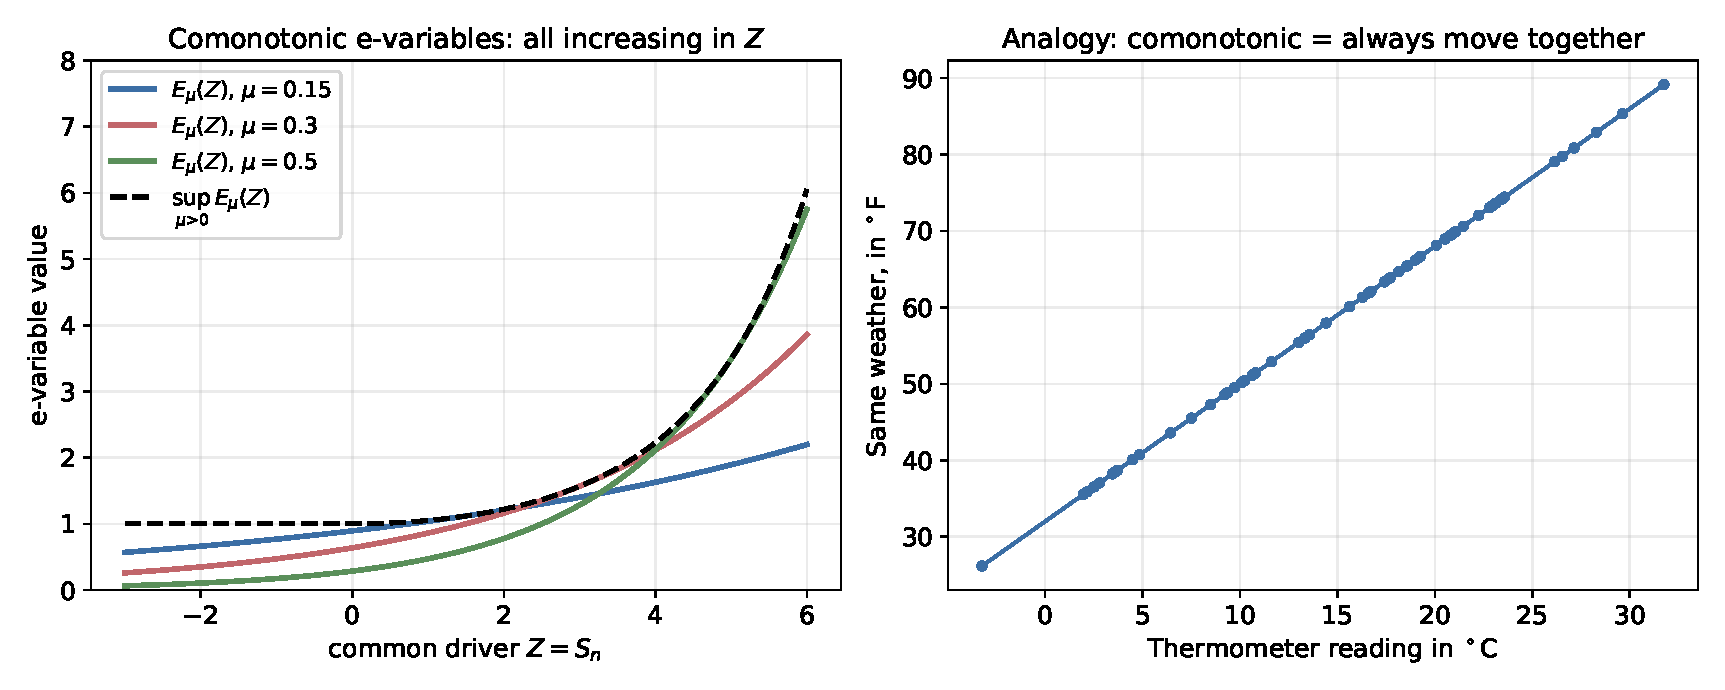
\includegraphics[width=0.98\linewidth]{fig_comonotonic.pdf}\\
  \small Left: the family $E_\mu(Z)=\exp(\mu Z - n\mu^2/2)$ for several $\mu>0$, all increasing in the common driver $Z=S_n$, with envelope $\sup_{\mu>0}E_\mu(Z)$ (Example 15.6). Right: the thermometer analogy -- two rescalings of the same underlying quantity always move together.
\end{frame}

%% =========================================================================
\begin{frame}{Section 15.3 -- Intuition: density conditions}
  \begin{itemize}
    \item A \textbf{density condition} is an assumption that the e-value's distribution has a well-behaved density -- ruling out the pathological, spiky/atomic worst-case distributions that make the plain Markov bound tight.
    \item Recall: the worst-case e-variable for Markov's inequality puts \emph{all} its mass at exactly two points ($0$ and $1/\alpha$) -- extremely spiky. If we know $E$ has, say, a \emph{decreasing} density (most mass concentrated near small values, smoothly tapering off, as with an Exponential or Pareto variable), that spiky worst case is structurally impossible.
    \item \textbf{Punch line of this section:} a decreasing (or unimodal) density on the e-value lets us cut the rejection threshold roughly \emph{in half}: instead of $1/\alpha$, we can reject at about $1/(2\alpha)$ -- a substantial, checkable power gain, for a mild and often plausible shape assumption.
  \end{itemize}
\end{frame}

%% =========================================================================
\begin{frame}[allowframebreaks]{15.3 Density conditions}
  \begin{block}{Three shape-constrained classes}
    \[
      \ED = \{E\in\frakE : E \text{ has a decreasing density on its support}\},
    \]
    \[
      \EDone = \{E\in\frakE : E \text{ has a decreasing density over } [1,\infty)\},
    \]
    \[
      \EU = \{E\in\frakE : E \text{ has a unimodal density on } [0,\infty)\}.
    \]
    A density on $[0,\infty)$ is \emph{unimodal} if it increases on $[0,x^\star]$ and decreases on $[x^\star,\infty)$ for some mode $x^\star\ge0$ (point masses at the mode are allowed). Note $\ED\subseteq\EU$, so $R_\gamma(\EU)\ge R_\gamma(\ED)$. Decreasing densities cover, e.g., Exponential and Pareto e-variables; unimodal densities additionally cover Log-normal and Gamma. These are conditions on the e-value's \emph{own} distribution, not on the hypotheses being tested.
  \end{block}

  \begin{block}{Theorem 15.7: the improved bounds}
    For $\gamma\in(0,1]$:
    \begin{enumerate}
      \item[(i)] $R_\gamma(\ED)=\gamma/2$ for $\gamma\ne1$, and $R_1(\ED)=1$;
      \item[(ii)] $R_\gamma(\EDone) = \gamma\big/\big(1+\sqrt{1-\gamma^2}\big)$;
      \item[(iii)] $R_\gamma(\EU) = (\gamma/2)\vee(2\gamma-1)$.
    \end{enumerate}
  \end{block}

  \framebreak

  \begin{block}{Step-by-step derivation of $R_\gamma(\ED)=\gamma/2$ (part (i))}
    Fix $z>1$ and set $\gamma=1/z$ at the end. We seek $\sup_{E\in\ED}\PP(E\ge z)$ subject to $\EE^\PP[E]=1$ (validity) and a decreasing density.

    \textbf{Step 1 -- reduce to a two-parameter extremal family.} Among all decreasing-density $E$ with left endpoint of support at $0$, the one that maximizes $\PP(E\ge z)$ for fixed mean $1$ turns out to be a mixture of a point mass at $0$ (weight $1-w$) and a Uniform$[0,b]$ density (weight $w$), for some $b\ge z$. (Intuition: moving density mass \emph{away} from the middle, either down to $0$ or spread thin near the tail cutoff $z$, only helps push more mass past $z$ while respecting ``decreasing density.'')

    \textbf{Step 2 -- impose the mean-1 constraint.} The mean of this mixture is $w\cdot(b/2)$ (point mass contributes $0$), so $\EE[E]=1$ forces $w = 2/b$.

    \textbf{Step 3 -- write down $\PP(E\ge z)$ and optimize over $b$.}
    \[
      \PP(E\ge z) = w\cdot\frac{b-z}{b} = \frac{2}{b}\cdot\frac{b-z}{b} = \frac{2(b-z)}{b^2}.
    \]
    Differentiate in $b$ and set to $0$: $\dfrac{\mathrm d}{\mathrm db}\Big[\dfrac{2(b-z)}{b^2}\Big]=\dfrac{2(2z-b)}{b^3}=0 \implies b^\star = 2z$.

    \textbf{Step 4 -- plug back in.} At $b^\star=2z$: $w^\star = 2/(2z)=1/z$, and
    \[
      \PP(E\ge z) = \frac{2(2z-z)}{(2z)^2} = \frac{2z}{4z^2} = \frac{1}{2z}.
    \]
    \textbf{Step 5 -- translate to $\gamma$.} Set $z=1/\gamma$: $\PP(E\ge1/\gamma)=\gamma/2$. This is attained (mean checks out: $w^\star b^\star/2 = (1/z)(2z)/2=1$), so
    \[
      R_\gamma(\ED) = \gamma/2, \qquad \gamma\ne1.
    \]
  \end{block}

  \framebreak

  \begin{block}{Reading off the improved threshold}
    Inverting $R_\gamma(\ED)=\gamma/2=\alpha$ gives $\gamma=2\alpha$, hence
    \[
      T_\alpha(\ED) = \frac{1}{2\alpha}.
    \]
    \textbf{Main message:} when an e-variable is known to have a decreasing density, its rejection threshold can be \emph{boosted by a factor of exactly $2$} relative to the naive $1/\alpha$ -- for every $\alpha$, not just asymptotically. The same factor-of-roughly-$2$ message holds for $\EDone$ (for small $\alpha$, $T_\alpha(\EDone)\approx T_\alpha(\ED)+\alpha/2$) and for $\EU$ (in the practically relevant range $\gamma\le2/3$, i.e.\ $\alpha\le1/3$).
  \end{block}

  \begin{block}{A meta-lesson worth remembering}
    For small $\alpha$, the shape of the e-value's distribution \emph{near $0$} (the ``uninformative'' region) barely affects the rejection threshold -- what matters almost entirely is the shape of the \emph{tail}, i.e.\ how the density behaves for \emph{large} e-values. This is why a tail-shape assumption like ``decreasing/unimodal density'' is exactly the right kind of extra information to exploit.
  \end{block}
\end{frame}

%% =========================================================================
\begin{frame}{Figure: worst-case type-I error under density conditions}
  \centering
  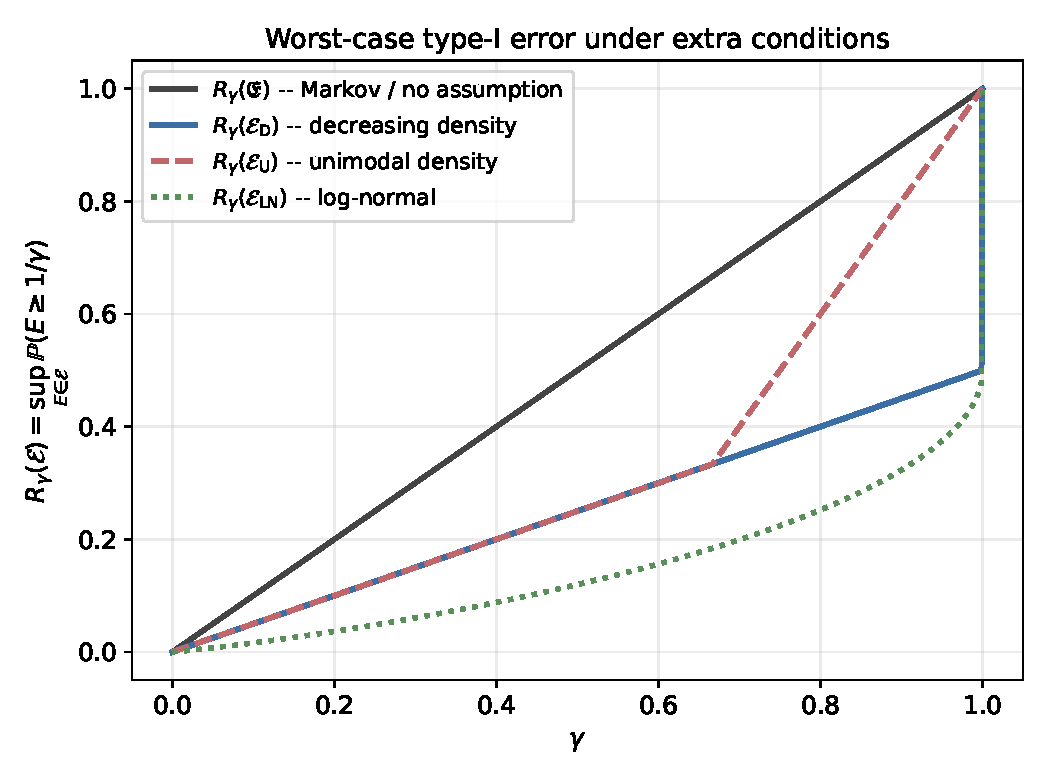
\includegraphics[width=0.78\linewidth]{fig_Rgamma.pdf}\\
  \small $R_\gamma(\calE)$ vs.\ $\gamma$: the diagonal is the plain Markov bound ($\calE=\frakE$); decreasing density ($\ED$) and unimodal density ($\EU$) both roughly halve the worst-case probability of a large e-value, especially for small $\gamma$. The log-normal curve ($\ELN$, from Section 15.4) is even lower.
\end{frame}

%% =========================================================================
\begin{frame}{Figure: the resulting improved thresholds}
  \centering
  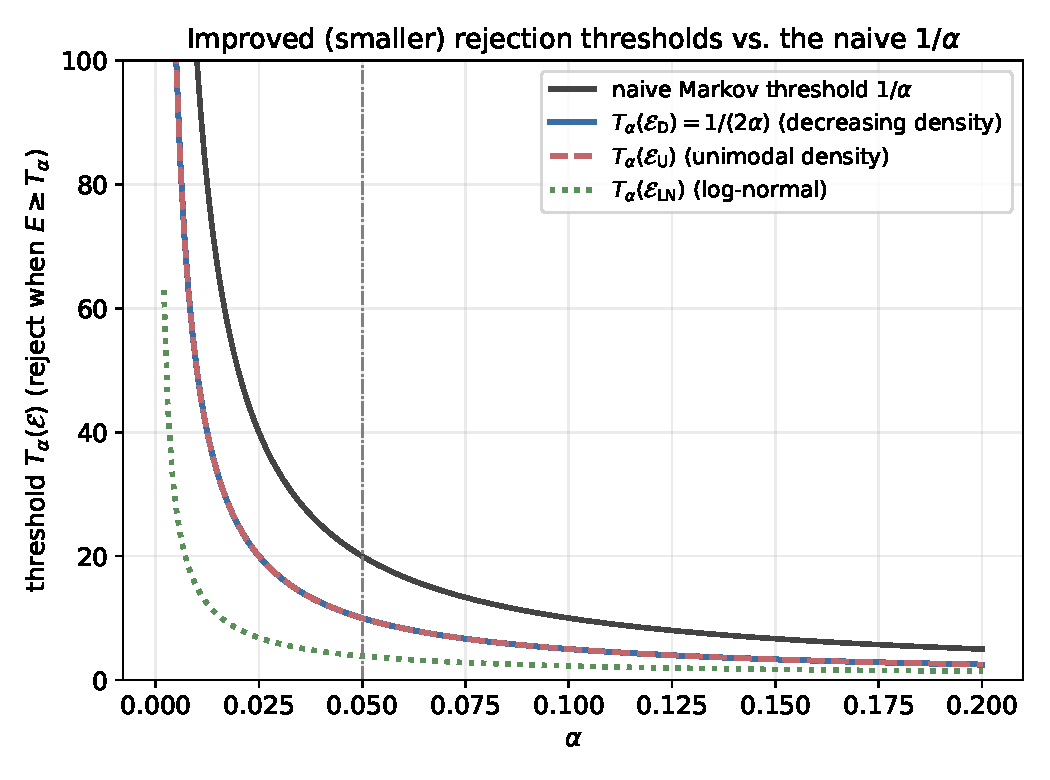
\includegraphics[width=0.78\linewidth]{fig_Talpha.pdf}\\
  \small $T_\alpha(\calE)$ vs.\ $\alpha$: the naive Markov threshold $1/\alpha$ (black) compared against the improved (smaller, less conservative) thresholds under a decreasing density ($T_\alpha(\ED)=1/(2\alpha)$), a unimodal density, and a log-normal distribution. The vertical line marks $\alpha=0.05$, our running numerical example.
\end{frame}

%% =========================================================================
\begin{frame}[fragile]{Python: verifying the decreasing-density bound (15.3)}
  \begin{lstlisting}
import numpy as np
rng = np.random.default_rng(2)

alpha = 0.05
naive_T = 1 / alpha                 # = 20
improved_T = 1 / (2 * alpha)        # = 10, Theorem 15.7(i)

reps = 3_000_000

# Two DIFFERENT decreasing-density e-variables in E_D, both with mean 1:
# (a) Exponential(1): density e^{-x} on [0, infty), strictly decreasing.
E_exp = rng.exponential(scale=1.0, size=reps)

# (b) Pareto-type: point mass 1-w at 0, Uniform[0,b] w.p. w (the EXTREMAL
#     family from the Theorem 15.7(i) derivation), with b = 2*improved_T,
#     w = 1/improved_T  -- this is the worst case, so it should ATTAIN gamma/2.
b = 2 * improved_T
w = 1 / improved_T
mask = rng.uniform(0, 1, reps) < w
E_extremal = np.where(mask, rng.uniform(0, b, reps), 0.0)

for name, E in [("Exponential(1)", E_exp), ("Extremal mixture", E_extremal)]:
    p_naive = (E >= naive_T).mean()
    p_improved = (E >= improved_T).mean()
    print(f"{name:18s}: P(E>=1/alpha)={p_naive:.5f}  P(E>=1/(2alpha))={p_improved:.5f}"
          f"  (target R_gamma(E_D) = alpha/2 = {alpha/2:.5f})")
# Both respect P(E >= 1/(2 alpha)) <= alpha/2; the extremal mixture attains it with equality.
  \end{lstlisting}
\end{frame}

%% =========================================================================
\begin{frame}{Running example, part 1: setup (coin-fairness style)}
  \begin{block}{Recall the coin-fairness running example (cf.\ Chapter 3)}
    Coin flips $X_i\in\{-1,+1\}$ ($X_i=+1$ for heads with probability $p$), so $\EE[X_i]=2p-1=:\mu$. Under $H_0$ ($p=1/2$, fair coin), $X_i$ has mean $0$ and variance $1$. By the CLT, for moderately large $n$ the sum $S_n=\sum_{i=1}^n X_i$ is approximately $N(0,n)$ -- so the Gaussian likelihood-ratio e-variable of Example 15.6,
    \[
      E_\mu = \exp\big(\mu S_n - n\mu^2/2\big),
    \]
    is (approximately, via the CLT) a sequential e-variable for detecting a biased coin with bias $\mu=2p-1$.
  \end{block}
  \begin{block}{A key structural fact: $E_\mu$ is exactly log-normal under $H_0$}
    Under $H_0$, $S_n\sim N(0,n)$ (in the Gaussian/CLT approximation), so
    \[
      \log E_\mu = \mu S_n - n\mu^2/2 \sim N\big({-n\mu^2/2},\,n\mu^2\big).
    \]
    That is, $E_\mu$ has a \emph{log-normal} distribution: $E_\mu\in\ELN$ (Section 15.4). Since log-normal densities are unimodal, also $E_\mu\in\EU$ (Section 15.3). This single e-variable is thus a perfect vehicle for the improved thresholds of \emph{both} sections.
  \end{block}
  \begin{block}{The naive threshold}
    At $\alpha=0.05$: naive Markov threshold $=1/\alpha=20$.
  \end{block}
\end{frame}

%% =========================================================================
\begin{frame}{Running example, part 2: improved thresholds \& how much power they buy}
  \begin{block}{Step 1: the improved thresholds at $\alpha=0.05$}
    \begin{itemize}
      \item Decreasing/unimodal density (Theorem 15.7): $T_\alpha(\ED)=1/(2\alpha)=\mathbf{10}$ -- exactly half the naive threshold.
      \item Log-normal (Theorem 15.10(v), since $R_\gamma(\ELN)=\Phi(-\sqrt{-2\log\gamma})$): solving $\Phi(-\sqrt{-2\log\gamma})=0.05$ numerically gives $\gamma^\star\approx0.2585$, so $T_\alpha(\ELN)=1/\gamma^\star\approx\mathbf{3.87}$ -- more than $5\times$ smaller than naive!
    \end{itemize}
  \end{block}
  \begin{block}{Step 2: what this buys in power (fixed $\mu=0.2$, i.e.\ $p=0.6$, $n=100$ flips)}
    Reject when $S_n \ge S^\star(T):=\log(T)/\mu + n\mu/2$. Under the true bias $\mu=0.2$, $S_n\sim N(n\mu, n)=N(20,100)$ (CLT approx.), so power $=1-\Phi\big((S^\star(T)-20)/10\big)$:
    \begin{center}
    \begin{tabular}{lccc}
      \toprule
      Threshold used & $T$ & critical $S^\star(T)$ & power against $\mu=0.2$ \\
      \midrule
      naive Markov ($1/\alpha$) & $20$ & $24.98$ & $30.9\%$ \\
      decreasing density $\ED$ & $10$ & $21.51$ & $44.0\%$ \\
      log-normal $\ELN$ & $3.87$ & $16.76$ & $62.7\%$ \\
      \bottomrule
    \end{tabular}
    \end{center}
  \end{block}
  \begin{block}{Take-away}
    Same exact type-I error control ($\alpha=0.05$), yet knowing $E_\mu$'s shape (unimodal, or exactly log-normal) roughly \textbf{doubles}, then \textbf{doubles again}, the power against a fixed real bias -- purely from a shape assumption, with no extra data.
  \end{block}
\end{frame}

%% =========================================================================
\begin{frame}{Figure: the power gain, visualized}
  \centering
  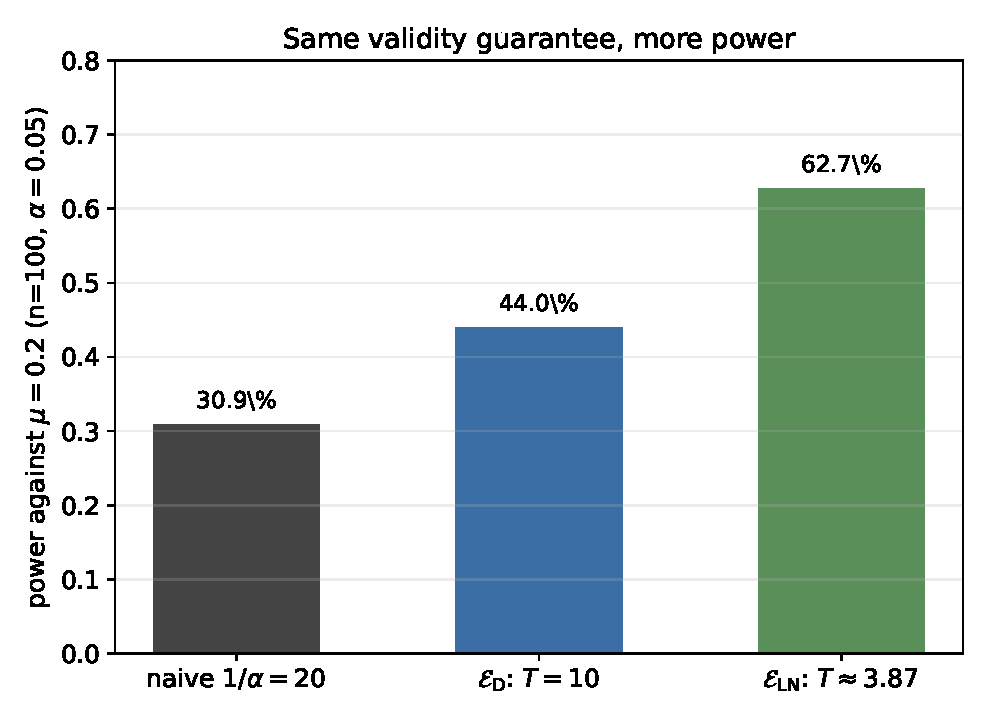
\includegraphics[width=0.62\linewidth]{fig_power_bars.pdf}\\
  \small Power against $\mu=0.2$ ($n=100$, $\alpha=0.05$) using the naive threshold vs.\ the improved thresholds from the density condition ($\ED$) and the log-normal condition ($\ELN$). Same validity guarantee throughout -- only the threshold (hence the power) changes.
\end{frame}

%% =========================================================================
\begin{frame}{Section 15.4 -- Intuition: why look at $\log E$ instead of $E$?}
  \begin{itemize}
    \item Many e-values used in practice are \emph{products} of many small per-observation e-values (e-processes, Chapter 7). A product's \emph{logarithm} is a \emph{sum} -- and sums of many small, roughly-independent pieces tend towards Gaussian-like shapes by the Central Limit Theorem.
    \item So instead of assuming a density condition directly on $E$ (Section 15.3), it is often more natural/plausible to assume a shape condition on $\log E$: e.g., that $\log E$ is symmetric, unimodal, or itself has a decreasing density.
    \item \textbf{Surprising subtlety:} not every such assumption on $\log E$ actually helps! Assuming $\log E$ is merely \emph{symmetric}, or merely \emph{unimodal} (without more), turns out to give \emph{no improvement at all} over the naive $1/\alpha$ threshold, in the practically relevant range. You need slightly more structure (decreasing density of $\log E$, or both unimodal \emph{and} symmetric, or exactly log-normal) to see a real gain.
  \end{itemize}
\end{frame}

%% =========================================================================
\begin{frame}[allowframebreaks]{15.4 Conditions on log-transformed e-variables}
  \begin{block}{Six classes (all require $\PP(E=0)=0$ so that $\log E$ is real-valued)}
    \[
      \ELS = \{E : \log E \text{ symmetric}\}, \quad
      \ELU = \{E : \log E \text{ unimodal density}\},
    \]
    \[
      \ELDzero = \{E : \log E \text{ decreasing density on } [0,\infty)\}, \quad
      \ELD = \{E : \log E \text{ decreasing density}\},
    \]
    \[
      \ELUS = \{E : \log E \text{ unimodal \emph{and} symmetric}\}, \quad
      \ELN = \{E : E \text{ log-normal}\}.
    \]
    A random variable $X$ is \emph{symmetric} if $X\stackrel{d}{=}c-X$ for some constant $c$. Containments: $\ELN\subseteq\ELUS\subseteq\ELS$ and $\ELD\subseteq\ELDzero$. ($E\in\frakE$ is log-normal iff $\log E\sim N(\mu,\sigma^2)$ with $\mu+\sigma^2/2\le0$, the constraint needed for $\EE[E]\le1$.)
  \end{block}

  \begin{block}{Theorem 15.10: the improved bounds}
    For $\gamma\in(0,1]$:
    \begin{enumerate}
      \item[(i)] $R_\gamma(\ELS)=\gamma\wedge(1/2)$ for $\gamma\ne1$ ($R_1=1$) -- \textbf{no improvement} for $\gamma\le1/2$ (i.e., essentially always in practice);
      \item[(ii)] $R_\gamma(\ELU)=\gamma$ -- \textbf{no improvement at all}, ever;
      \item[(iii)] $\gamma/(\mathsf{e}-\gamma) \le R_\gamma(\ELDzero) = \mathsf{e}^{-a_\gamma} \le \gamma/(1+\sqrt{1-\gamma^2})$, where $a_\gamma$ solves $\mathsf{e}^a(1-a-\log\gamma)=1$;
      \item[(iv)] $R_\gamma(\ELD)=R_\gamma(\ELUS)$, and $\gamma/\mathsf{e} \le R_\gamma(\ELD) \le \big(\gamma/(\mathsf{e}(1-\gamma^2))\big)\wedge\big(\gamma/(1+\sqrt{1-\gamma^2})\big)$;
      \item[(v)] $R_\gamma(\ELN) = \Phi\big(-\sqrt{-2\log\gamma}\big) \le \gamma/\big(2\sqrt{-\pi\log\gamma}\big)$, for $\gamma\ne1$ ($R_1=1$); $\Phi$ is the standard normal cdf.
    \end{enumerate}
  \end{block}

  \framebreak

  \begin{block}{Why (i) and (ii) are cautionary tales}
    Symmetry or unimodality of $\log E$ \emph{alone} says nothing about how thin the tail is -- $\log E$ could still have an extremely heavy (or even non-decreasing near its mode, spread-out) tail consistent with symmetry/unimodality, reproducing the worst-case Markov scenario. \textbf{Lesson:} vague shape words are not enough; you need an assumption that actually constrains the tail, such as a genuinely \emph{decreasing} density (of $\log E$ or of $E$ itself), or the fully parametric log-normal assumption.
  \end{block}

  \begin{block}{Why (iii)--(v) do help: roughly a factor of $\mathsf{e}\approx2.718$}
    For small $\gamma$, $R_\gamma(\ELDzero)$, $R_\gamma(\ELD)=R_\gamma(\ELUS)$ all behave like $\gamma/\mathsf{e}$ -- i.e., $T_\alpha(\calE)\approx \mathsf{e}/\alpha$ is \emph{wrong}; correctly inverting, the threshold shrinks by a factor of roughly $\mathsf{e}$ relative to $1/\alpha$ for small $\alpha$. The \emph{log-normal} assumption (v) is the strongest of all: $R_\gamma(\ELN)\to0$ much faster than linearly in $\gamma$ as $\gamma\to0$ (note the $\sqrt{-\log\gamma}$ inside $\Phi$), giving by far the smallest threshold of every class in this chapter.
  \end{block}

  \begin{block}{Connecting back to Section 15.3}
    $\ELDzero\subseteq\EDone$ (a decreasing-density-of-log condition on $[0,\infty)$ implies the raw variable has a decreasing density on $[1,\infty)$, since $\log E\ge0 \iff E\ge1$) -- so the two sections' results are genuinely compatible refinements of each other, not competing theories.
  \end{block}
\end{frame}

%% =========================================================================
\begin{frame}{Table 15.12: improved thresholds $T_\alpha(\calE)$ (reproduced)}
  \centering
  \small
  \begin{tabular}{lcccccc}
    \toprule
     & \multicolumn{6}{c}{$\alpha$} \\
    \cmidrule(lr){2-7}
    Class & $0.001$ & $0.01$ & $0.02$ & $0.05$ & $0.1$ & $0.2$ \\
    \midrule
    $\frakE,\ \ELS$        & $1000$   & $100$   & $50$    & $20$   & $10$  & $5$ \\
    $\ED,\ \EU$            & $500$    & $50$    & $25$    & $10$   & $5$   & $2.5$ \\
    $\EDone$               & $500$    & $50.01$ & $25.01$ & $10.03$& $5.05$& $2.60$ \\
    $\ELUS,\ \ELD$         & $367.88$ & $36.82$ & $18.45$ & $7.49$ & $3.93$& $2.25$ \\
    $\ELDzero$             & $368.25$ & $37.16$ & $18.77$ & $7.73$ & $4.07$& $2.25$ \\
    $\ELN$                 & $118$    & $14.97$ & $8.24$  & $3.87$ & $2.27$& $1.42$ \\
    \bottomrule
  \end{tabular}
  \vspace{1em}

  \small Reading the $\alpha=0.05$ column: naive $20$ (row 1) $\to$ $10$ (density condition) $\to$ $7.49$ (log-transform, decreasing/unimodal-symmetric) $\to$ $3.87$ (log-normal) -- each additional, checkable shape assumption buys a further reduction in the rejection threshold, i.e.\ more power at the same validity level.
\end{frame}

%% =========================================================================
\begin{frame}[fragile]{Python: log-transform thresholds and Table 15.12 (15.4)}
  \begin{lstlisting}
import numpy as np
from scipy.stats import norm
from scipy.optimize import brentq

def R_gamma_LN(gamma):
    """Theorem 15.10(v): R_gamma(E_LN) = Phi(-sqrt(-2 log gamma))."""
    return norm.cdf(-np.sqrt(-2 * np.log(gamma)))

def T_alpha_LN(alpha):
    """Invert R_gamma(E_LN) = alpha for gamma, then T = 1/gamma."""
    gamma_star = brentq(lambda g: R_gamma_LN(g) - alpha, 1e-9, 1 - 1e-9)
    return 1 / gamma_star

for alpha in [0.001, 0.01, 0.02, 0.05, 0.1, 0.2]:
    naive = 1 / alpha
    T_LN = T_alpha_LN(alpha)
    print(f"alpha={alpha:<6} naive=1/alpha={naive:8.2f}   T_alpha(E_LN)={T_LN:7.3f}"
          f"   improvement factor = {naive / T_LN:5.2f}x")
# Reproduces Table 15.12's E_LN row, e.g. alpha=0.05 -> T ~ 3.87 (a ~5.2x
# reduction versus the naive Markov threshold of 20).
  \end{lstlisting}
\end{frame}

%% =========================================================================
\begin{frame}{Chapter 15 summary}
  \begin{itemize}
    \item The plain Markov threshold $1/\alpha$ (Chapter 2) is tight only against a pathological, spiky worst-case e-variable. Restricting to a shape-constrained class $\calE\subsetneq\frakE$ lets us compute a strictly smaller, valid threshold $T_\alpha(\calE)\le1/\alpha$ (Section 15.1, Lemma 15.1).
    \item \textbf{Comonotonicity} (15.2): if a family of e-variables all move together (increasing functions of one common $Z$), their \emph{supremum} obeys the same tail bound as any single member (Lemma 15.4, Proposition 15.5) -- letting you use the best-fitting member of a parametric family (e.g., an MLE-based likelihood ratio) at no cost to validity.
    \item \textbf{Density conditions} (15.3): a decreasing or unimodal density on $E$ itself roughly \emph{halves} the threshold ($T_\alpha(\ED)=1/(2\alpha)$, Theorem 15.7) -- derived via an explicit worst-case mixture (point mass $+$ uniform tail).
    \item \textbf{Log-transform conditions} (15.4): shape assumptions on $\log E$ (motivated by products of e-values / CLT) can shrink the threshold by roughly a factor of $\mathsf{e}$ (decreasing density, or unimodal+symmetric) or dramatically more (exactly log-normal) -- but symmetry or unimodality of $\log E$ \emph{alone} gives no improvement (Theorem 15.10).
    \item \textbf{Running numeral:} testing a coin's bias ($\mu=0.2$, $n=100$, $\alpha=0.05$), the naive threshold $20$ gives power $30.9\%$; the density-condition threshold $10$ gives power $44.0\%$; the log-normal threshold $3.87$ gives power $62.7\%$ -- all with exactly the same $\alpha=0.05$ type-I error guarantee.
  \end{itemize}
\end{frame}

%% =========================================================================
\begin{frame}{Bibliographical note}
  \begin{itemize}
    \item This chapter is largely based on Blier-Wong and Wang [2024], where full proofs of all results (including the omitted proofs of Theorems 15.7(ii)--(iii) and 15.10) can be found, along with extensions to combined e-values and the e-BH procedure.
    \item General background on probability bounds under distributional shape information: Shaked and Shantikumar [2007], R\"uschendorf et al.\ [2024].
    \item Comonotonicity (Section 15.2) is a central concept in dependence modeling and in decision theory under ambiguity, via its connection to Choquet integrals [Schmeidler, 1989]. A standard reference is Denneberg [1994].
  \end{itemize}
\end{frame}

\end{document}
